\documentclass[pageno]{jpaper}

\newcommand{\IWreport}{2015}
\newcommand{\source}[1]{\caption*{Source: {#1}} }

\usepackage[normalem]{ulem}

\usepackage{graphicx}
\usepackage[english]{babel}
\usepackage{hyperref}

\setlength\parindent{24pt}

\begin{document}

\title{
Solar Source: A general framework for evaluating rooftop solar potential\\
Version 20151109v1}

\author{Graham Turk '17\\Adviser: Alan Kaplan}

\date{}
\maketitle

\thispagestyle{empty}
\doublespacing
\begin{abstract}
This document is intended to serve as a sample you can use for independent work reports.  We provide some guidelines on content and formatting.  They are not required, but they might be helpful.
\end{abstract}


\section{Introduction}  
Fossil fuel based electricity production is responsible for over one quarter of greenhouse gas emissions, acknowledged by the IPCC as the primary driver for global climate change ~\cite{IPCC}. Despite the shrinking cost of solar panels, solar photovoltaic (PV) energy, a renewable source, accounts for only 0.4\% of all US electricity \cite{USEIA}. Yet a solar installation can yield savings on electricity and reduce greenhouse gas emissions. New financing options like SolarCity's SolarPPA, which requires no upfront cost, are removing the economic barriers to installing solar.

If a homeowner today were interested in installing solar panels, she would likely hire a contractor to perform a site evaluation. The process is time-consuming and relies on the moral character of the contractor to give an honest estimate. The problem: homeowners don't have a free, simple, and accurate method to determine whether their homes are good candidates for a solar installation. With a bevy of open-source data on solar irradiance and electricity prices, the process should be easy. Motivated by a mission to reduce fossil fuel-based electricity generation, our goal is to provide every homeowner with a general framework to accurately compute the home's solar potential, the electricity generating potential and subsequent cost-savings potential of installing solar panels.

A general framework entails an adaptable software architecture and access to the methods used to produce the final result. It has the benefit of flexibility and transparency; other developers can augment the framework with custom modules and the homeowner can trace through the analysis. In building this framework we hope to help uncover the financial benefits of solar energy and get people aware of their rooftop generating potential. If adopted on a wide scale, this could prompt an ideological shift from grid to rooftop and from fossil fuels to the sun. With our framework, if a homeowner were interested in installing solar, she would launch the SolarSource application, input data specific to her home, and immediately receive an estimate for how much she could save by installing a solar array based on her roof availability and electricity consumption. We also envision that solar panel providers could use SolarSource to identify areas with high solar potential to better inform their marketing efforts. Perhaps a future commercial version of our framework would link up the prospective homeowners with the solar providers directly.

The remainder of this paper is organized as follows: first we will discuss some related work in solar potential mapping software and real-time performance modeling. Based on the gaps in previous work we will introduce our approach to solve the problem we identified. With the approach laid out, we will then describe the implementation of the SolarSource framework, an Android mobile application and Node.js RESTful API. Finally we will explain the methods used to evaluate the success of our approach and offer opportunities for future work. We view locally generated renewable electricity as an essential step towards global decarbonization, a major aspect of climate change mitigation. A user-friendly framework to evaluate a home's solar potential is a first step in that direction.

\section{Related Work}
\subsection{Project Sunroof}
Many commercial apps have been built to answer the question``how much could I save by installing solar panels?'' Until recently, however, most of those systems were either simple calculators that provide simplistic estimates or complicated applications that require specialized knowledge of solar panels. Then in April 2015, Google released Project Sunroof. The web application takes an address an input, then combines a 3D model of your house with weather data to generate a roof analysis. Using the roof analysis and your monthly electricity bill (the only other input to the process), it recommends a solar installation to generate approximately 100\% of your home's electricity use. The service tax credits, utility rebates and renewable energy credits to calculate the final cost of the array. Comparing the price of the installation to projected electricity costs (with options to buy, lease, or purchase via loan), Sunroof estimates savings over a 20-year period. It also allows the user to share the savings estimate with selected solar providers, presumably to help providers market effectively. Project Sunroof's simple interface and minimal user input stood out as two features we wished to emulate. Figure \ref{fig:sunroof} shows 

\begin{figure}[h]
\begin{center}
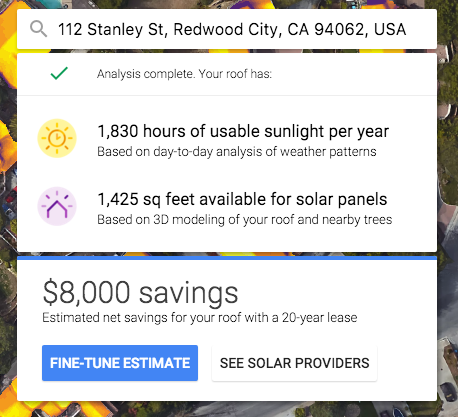
\includegraphics[scale=0.5] {sunroof}
\caption{Project Sunroof analysis and estimated savings for California address with \$100 per month electricity bill}\label{fig:sunroof}
\end{center}
\end{figure}

Though at first Project Sunroof seemed to solve the problem we set out to address, we quickly learned that it fell short in several key areas. When we typed in my own home addresses to calculate the estimated savings, we discovered that Project Sunroof was not available in any of our home states, covering only Fresno, the San Francisco Bay Area, and Boston (Project Sunroof has since expanded coverage to 7 more cities in the United States). Using a sample address, we investigated the calculations Google used to produce the final recommendation. The algorithm uses a fixed loan interest rate (5.0\%) and assumes a utility electricity price increase of 2.2\% per year. Furthermore it assumes that electricity consumption will remain the same for 20 years, only permits monthly bill values in \$50 increments, and sets a seemingly arbitrary upper limit on monthly bill of \$500, unrelated to available roof area \cite{Sunroof}. 

Even more notable, when we compared the production of the recommended solar array size to the home's current consumption (the monthly electricity cost divided by the regional price for electricity on a dollar per kWh basis) I discovered that Project Sunroof assumes the panels generate at peak output for up to 100\% of daylight hours. To clarify, that would mean that the sun is at its peak for all daylight hours, which even in sunny California is not the case. As software developers, we saw it as an issue that we could not access the data from the analysis through an API; the results were only available through Google's interface. From our early analysis, Project Sunroof stood out as a rigid, single-interface app. While it does provide an estimate for the home's solar potential and help spread the word of the benefits of rooftop PV, it uses fixed assumptions and a generic monthly electricity consumption total unadaptable to patterns of electricity use. Despite its good intentions, it leaves gaps in its solution to the problem we set out to address.

\indent The ``100\% recommendation'' by many commercial savings calculators also runs the risk of misleading the user. An installation to cover 100\% of electricity consumption doesn't mean that the home can disconnect from the grid; it means that the solar array's total generation matches the home's total consumption. Yet without an energy storage system the home must remain connected to the grid for times when the sun isn't shining.

Similar to Project Sunroof, a study in the journal Computers, Environmental and Urban Systems explored techniques to determine available rooftop area for photovoltaic deployment in Ontario, Canada. The comprehensive study uses a five-step procedure involving geographic division of the region and shading reduction. It concludes that 30\% of Ontario's electricity demand could be met with province-wide PV deployment \cite{Wiginton2010345}. Studies like this one are important for utility planning, but they do not address individual homeowner interests. The software was used to produce a static result, not published as a tool for homeowners to use for future evaluations.

In our study of Project Sunroof, we recognized that the overall monthly bill might not provide a complete view of a home's electricity consumption. The DOE released a tool called the Green Button that allows utility customers to download detailed reports of their energy consumption. The initiative is intended to allow the utility customers to take advantage of online applications to help them manage energy use and save on bills. Included in the examples of such applications are products and services for ``sizing and financing rooftop solar panels.'' Although we did not ultimately implement an analysis tool to look at detailed patterns of electricity use as part of the recommendation, a developer could augment our pluggable framework with data from Green Button in a more advanced iteration of the energy model.

In examining available open source data in the solar mapping field, the National Renewable Energy Laboratory (NREL) appeared frequently as a data source in commercial applications. NREL's Solar Prospector is a mapping tool for commercial and utility scale solar projects \cite{Prospector}. Although the prospector does not have rooftop-specificity (instead displaying broad solar potential categories for large regions), it uses other NREL services available through developer APIs. We found services for the solar pricing landscape, nationwide utility prices, average irradiance values at a specific latitude and longitude, and future performance prediction; these services became core components of our implementation. Although the Solar Prospector does not consider the cost-competitiveness of a solar system by pricing comparison to grid electricity, NREL also released the System Advisor Model (SAM), a performance and financial model designed to ``facilitate decision making for people involved in the renewable energy industry.'' \cite{SAM}. SAM is a robust tool that makes performance predictions for solar PV and wind projects. We judged the platform to be overly complex for a prospective rooftop solar owner, intended more for installers than homeowners. 

\subsection{Performance Prediction}

There has been exciting work in the field of solar performance prediction. Researchers from the University of Massachusetts developed SolarCast, a cloud-based service that provides customized site-specific predictions of generation for solar deployments ~\cite{Iyengar:2014:SCB:2674061.2674071}. Funded by the Massachusetts Department of Energy Resources, SolarCast uses a "blackbox" approach that requires only i) a site's geographic location and ii) a minimal amount of historical generation data. While the software can predict future performance of a solar array, it does not give insights into a new installation. However, we identified performance prediction as an important part of our approach, both to evaluate the success of our approach (by simulating the generation of our recommended array) and potentially as part of the recommendation algorithm itself. Rather than using an assumed production value (1 kilowatt per square meter for example), we could use existing arrays as part of a crowdsourcing platform, using a performance prediction model like SolarCast on those arrays to predict the output of a hypothetical installation in a similar environment. After contacting the researchers involved with the project, we acquired a key to use the SolarCast alpha API. Although the API is still not yet ready for our use, our research on SolarCast led us to other performance prediction APIs, which we ultimately used to evaluate our approach, and real-time generation data, a core element of our implementation.

Also in the area of panel performance prediction, researchers from the University of Maryland built a solar panel emulation platform. SunaPlayer \cite{Bobovych:2015:SHE:2737095.2737110} uses a host of physical electronic devices to built a model of a solar panel. Despite its apparent relevance to our efforts, SunaPlayer is intended to aid with solar panel design, not as an evaluation metric for hypothetical installations. Nonetheless, the paper indicates to us the growing interest in software for solar PV applications. We hope that SunaPlayer and similar initiatives help eliminate doubt surrounding the performance of solar panels, thereby removing a barrier to further growth.

Panel performance prediction is just one half of the equation when determining the long-term cost effectiveness of a solar system. We also must consider the expected behavior of the utility market. eForecast, a prototype built by researchers at the Aalborg University in Denmark, seeks to supplement the data on current and past electricity usage with "eco-forecasting" ~\cite{Kjeldskov:2015:EDE:2702123.2702318}. The prototype forecasts expected usage, electricity price, and expected drops and peaks. It purports to enable people to use electricity at more opportune times. Though we were not granted permission to incorporate eForecast techniques into our algorithm, we designed our framework to allow future integration. eForecast and other prediction technologies could become important tools to inform our installation recommendation. \newline

\subsection{Real-time Monitoring Systems}
Companies like Bidgely, PlotWatt, and Wattvision monitor home electricity usage with sensors that mount onto electricity meters. Using the electricity data feed, the companies can offer suggestions on improving energy efficiency. While Bidgely can, for example, perform energy disaggregation to distinguish grid electricity from solar, none of these companies evaluate the home's potential to support solar. Recognizing that real-time electricity usage data could help construct an energy profile of the home for the solar evaluation, we contacted Wattvision, a Princeton-based startup, and received access to an actual home data stream for testing. Although we were not able to develop an analysis tool more advanced than a simple computation of daily and monthly consumption, we built the infrastructure to allow a Wattvision plug-in to construct a home energy profile.

Related to real-time consumption monitoring is software for monitoring real-time solar panel performance. Many solar providers including SunPower, Enphase, and First Solar provide APIs and interfaces for their customers to access real-time performance of their arrays. For example, live electricity generation from Princeton University's solar array is available through SunPower's API and visualized in the Office of Sustainability's Tiger Energy app. After surveying solar systems, we chose the Enphase Enlighten system as the one for further analysis because of its extensive API. The Enlighten API has endpoints to fetch current production, total monthly production, and power per area \cite{Enlighten}. Although the API is principally intended for Enlighten customers to access their own data, they provide a mechanism to allow third-party developers to request access to data feeds. We reached out to a member of the Enphase developer team, who identified a group of candidate systems that could produce an accurate estimate for the power output of a hypothetical array. We are currently awaiting final approval to send out authorization requests, which will allow us to make API requests on behalf of real users to access their system data.

Considering the related work we studied, we identified Project Sunroof's model as an ideal medium for conveying the recommendation and savings estimate to the homeowner. Similar to Project Sunroof, we chose cost savings and installation size as the two key values to report to the user. When we began work on SolarSource we recognized three areas as missing from previous efforts in the "software-for-solar" field: universal coverage, adaptability, and incorporation of actual generation data. This led to our approach.

\section{Approach}
\subsection{Guiding Principles}
In formulating our approach, we were guided by the principles of transparency and flexibility. Our original goal was not only to provide the homeowner with a recommendation and savings estimate, but also to do so within a general framework, decoupled from the front end application and including transparent access to methodology, data sources, and analysis. To the best of our understanding, that model had never been executed before. 

A high level description of our approach: we construct a model of the home with electricity consumption data and a user-generated roof mapping. We use home model properties to make public third party API requests and incorporate crowdsourced generation data to create a rooftop solar profile of the home. We perform a financial analysis based on that integrated data model and return the result of the analysis to the user via a public API.

Five key ideas underlie the approach:
\begin{itemize}
\item decoupled back end: public API for flexible access to analysis tools
\item adaptable architecture: open source and pluggable code to allow custom modules
\item universal coverage: homeowners supply the data for energy and roof profiles
\item leverage 3rd party APIs: use public NREL services as core data sources
\item crowdsourced power generation data: incorporate actual array production values into recommendation
\end{itemize}

consumption-specific recommendations: electricity consumption patterns (acquired through a Wattvision monitor), rather than a generic monthly aggregate, inform our analysis
Future-centric
- we look at forecasted future weather data, as well as predicted performance of the array

\subsection{Decoupled Back End}
To enable widespread and flexible use of the framework, we decided to build the back end of the framework as a standalone API conforming to REST protocol. The benefit of such an approach is broader potential impact. With a publicly accessible API and a comprehensive JSON return output, anyone with knowledge of HTTP can make requests to the API to use our analysis tool, either a developer writing a front-end application or even a homeowner with specialized knowledge of her roof floor plan. The information we can provide is not limited to users of our Android application.

\subsection{Adaptable Architecture}
All of the software-for-solar apps we discovered in our research hide their implementations; we set out to create a useful tool for both homeowners and the developer community. To do that we decided to open-source the code on Github in a public repository. We designed the software to allow plug-in modules. Again here, the benefit of this approach is the potential scope of impact. With our code on Github, any curious user can walk through our analysis step by step. Furthermore, any developer can build on the work we started, augmenting the framework with custom modules or displaying it in a specialized interface.

As an example of one potential custom module, consider this: when examining Project Sunroof's methodology, we questioned whether a monthly electricity bill is sufficient for a comprehensive home electricity model. Our adaptable architecture enables a developer to write a module that constructs the home electricity profile from a Wattvision data stream or GreenButton report. Detailed readings of electricity consumption yield a precise view of the home's usage patterns to inform the analysis [useful information for a hypothetical solar installation]. If, for example, the home uses the majority of its electricity after sundown, then recommending an installation to cover 100\% of the home's consumption might be misguided depending on power purchasing agreements with the regional utility company. Another potential issue: electricity bills vary according to season. Typically the warmer months are associated with higher costs because of frequent air conditioning use. Based on audits of Long Island, NY electricity bills, the January bill could yield a recommended array size that covers under half the consumption in July. Wattvision or GreenButton provide meter readings over the whole year's span, yielding a more complete view of home consumption. Our insight to support a Wattvision data stream or GreenButton report to construct the home electricity profile helps avoid inaccuracy issues. To enhance generality, if the user does not have access to either of these data sources, we also provide the simple monthly bill format.

\subsection{Universal Coverage: Do-it-Yourself Home Profile}
An accurate model of the home is the foundation for any type of energy upgrade including a solar installation. Our goal is to provide {\em every homeowner} with the tools to determine the home's solar potential - to achieve that goal we needed to make the framework universally usable. After surveying previous work, we realized that we could construct an accurate profile of the home with user-supplied data on roof properties and electricity consumption. This technique permits the framework to be used anywhere with internet access, unlike Project Sunroof, whose utilization depends on Google's choice of coverage. Providing the user with the tools to profile the home severs our dependence on potentially out-of-date map APIs and electricity data. For example if a homeowner has recently built an extension to the home, an aerial image might not depict the current roof, leading to an inaccurate estimate of solar generating potential.

\subsection{Leverage Third-Party APIs}
In order to determine the generating capacity of a rooftop solar PV system, as well as the price of that system, we needed data on panel prices and sunlight availability at a specific location. Previous efforts have relied on proprietary data. Yet to achieve our goal of both an accurate {\em and} transparent framework, we required data that is both dependable and publicly accessible. From our study of NREL's Solar Prospector application, we learned that much of the data we needed is openly available through NREL's developer API. We decided to use NREL's datasets as the core informational foundation of our recommendation analysis. This decision has two key benefits. Firstly, as a governmental facility that has contributed to renewable energy developments since 1974, NREL is a reputable and reliable source. Secondly, the data is openly available; this allows other developers to augment our framework (by forking the project on Github, for example) without worrying about proprietary access issues. It also helps keep our methodology transparent, so that a curious homeowner could retrace the steps of our algorithm, fetching the data used each step for a clear understanding of how we generate the recommendation. 

\subsection{Crowdsource Power Generation Data}
The third key component of our approach is to use actual generation data when estimating the production of the recommended array. The accuracy of the recommendation relies heavily on the power output of the array. Some services use generic industry-reported values for a panel's output. However, production values vary depending on environment. Rather than using a fixed value, the power per area value in our analysis is computed using a collection of actual array sources. Using crowdsourced data from real installations close to the target address allows us to get a realistic view of how the panels would perform in practice.

------

\section{Implementation}
\subsection{Breakdown of the work}
The work on SolarSource was divided into three areas among our team (composed of Emily Speyer, Gregory Magana, and myself): roof profiling, core Android application, and back end API. Although my work is completely separate from the front end interface, we collectively chose to build a mobile app to facilitate ease of use and to take advantage of phone features like compass, camera, and GPS.

Emily implemented the roof profile as a standalone Android application that integrates with the core app. With the roof profiling system, the user maps out the roof's area by walking around the perimeter of the home. The program factors in shade and other obstructions to the roof to compute the usable roof area along with tilt angle and orientation. The roof profile provides the physical constraints for an installation and necessary parameters to determine how much electricity a hypothetical rooftop-mounted PV system could produce.

Gregory built the main Android application. It accepts user input on monthly electricity bill or Wattvision system identification numbers (to allow the back end to make Wattvision API requests for the analysis), delegates control to the roof profiling stage, and communicates with the RESTful API backend to compute and display the final recommendation. The home energy profile, created with data sent through an Android application, determines the cost-effectiveness of the proposed solar system. 

I implemented the back end API, which uses data from the front end to produce a recommended installation size and performs the cost analysis. First I will explain the high level design decisions behind the API. Then I will give an overview of my implementation and then discuss each step individually. 

\subsection{System Architecture}

\begin{figure}[h]
\begin{center}
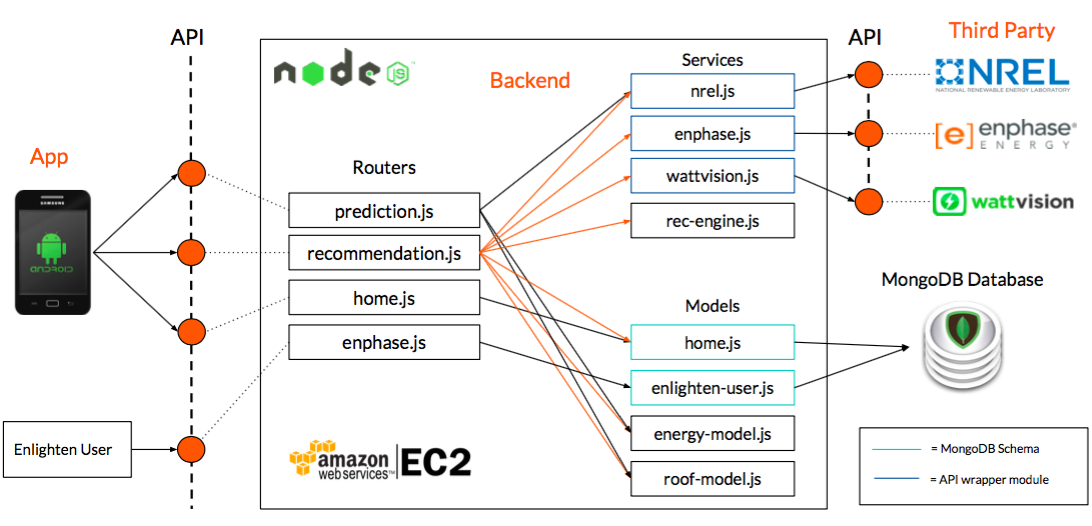
\includegraphics[width=\textwidth] {architecture}
\caption{High level implementation}
\label{fig:architecture}
\end{center}
\end{figure}

Figure \ref{fig:architecture} shows a high-level illustration of our architecture. The basic structure is as follows: we expose an API with endpoints to create a home model, retrieve the solar array recommendation and cost estimate, and simulate the future performance of the array for testing. The codebase consists of three file categories: routers, services, and models. Routers handle the HTTP request logistics, perform input validation, retrieve objects stored in the database, and call service methods. We gave each API category its own router to promote modularity. The models consist of both database schemas (descriptions of database objects) and home models created with input from the user. Services include wrapper modules to call third party API methods and the recommendation engine, which computes the necessary array size and performs an economic analysis to estimate savings. We store all home objects in a database. We chose MongoDB for the database layer and deployed the application to an Amazon Web Services EC2 instance.

\subsection{Platform and Web Framework}
The first decision we faced was which platform to use to build the API. Our goal in this step was to find a platform that promoted adaptability, facilitated HTTP routing and was enjoyable to program with. Popular approaches include Python (with the Django web framework) and Node.js (a Javascript-based runtime environment). We recognized that to achieve the flexibility goal from our approach we needed a platform that supported easy integration of custom modules. With that consideration, Node.js became the clear choice for its modular design and robust package manager, npm. Every file in Node is a module with associated methods and instance variables. Node's design aligned with our need to allow developers to plug in their own code without modifying large chunks of the original codebase. Our architecture presents opportunities for developers to write custom analytics tools in such areas as Wattvision stream parsing, electricity price forecasts, and future consumption predictions based on current patterns, an alternative to assuming constant consumption for 20 years.

With Node, installing an external package is as simple as one npm command; importing the package (or an internal module file) entails initializing a single variable, which scopes the entire package to that variable, a major benefit in light of Javascript's exclusively global namespace. In our architecture we created a module for each service file to conveniently package its functionality. Once we decided to use node, we downloaded the Node package using the OS X package manager Homebrew.

Next we needed to choose a web framework. Our goal in this step was to maximize code readability. We considered not only syntax but also popularity; the time it takes to read documentation on an unfamiliar framework hinders a developer's understanding of our code. We experimented with several popular and well-reviewed frameworks (writing basic route handlers with each one) including Loopback, Sails, and Express. Express is the most popular Node framework on Github and used in production by Netflix. Its documentation is well-written and contains many useful code examples. Loopback is a heavy-duty framework, providing features like automatic API documentation and support for Android applications. However, it is bloated with highly specialized functionality and convoluted syntax. More importantly, the documentation was difficult for us to understand, a key drawback for an approach guided by readability. Sails is inspired by Express and extends it for front end functionality. It is a full model-view-controller framework, intended for use by MVC applications. Given that the back end is solely an API, we decided to use the more minimalist Express, which was also the most straightforward to write route handlers in our experimentation. We used the npm package express-generator to create an Express template for the application. The template separates route handling functions in a separate folder, a structure we adhered to throughout development. After reading the Express documentation, we wrote the route handling methods for home creation, retrieval, update, and deletion.

\subsection{Callbacks vs Promises}
One decision we immediately faced was how to deal with asynchronous method calls. In Javascript, code does not execute sequentially. Asynchronous I/O and method calls do not block; instead execution jumps to the next line. To deal with this language feature, most programs make extensive use of callback functions, whereby you pass a function as an argument to an asynchronous method. The function is called with the response of the asynchronous request. As we read tutorial code, we decided that function callbacks made code difficult to understand. When asynchronous calls are nested, they can produce the dreaded and unreadable ``pyramid of doom'':

\begin{figure}[h]
\begin{center}
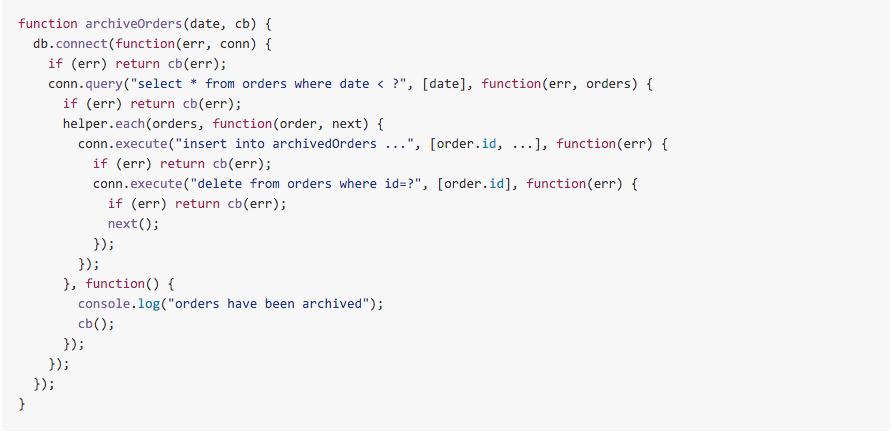
\includegraphics[scale=0.5] {callback-hell}
\caption{Pyramid of doom whereby the function grows outward as a result of many nested callbacks}
\label{fig:callback-hell}
\source{https://github.com/Sage/streamlinejs}
\end{center}
\end{figure}

We knew that our code would be open-source and we intended for it to be iterated on by other developers (forkable). To do that, it needs to be easily understood; readability should be the rule. Our goal in writing asynchronous Javascript was the same as in choosing a web framework: maximize readability. In light of that goal we determined that we couldn't use callbacks. 

There are numerous Node libraries to get around callbacks. We surveyed the options by looking at discussions on Stack Overflow and reading code samples to gauge readability and ease of use and discovered that the two primary high-level approaches to combat the callback model are callback replacement and promises. Callback replacement involves replacing the callback function with a special symbol and writing the code as if the function were synchronous. The replacement library handles the asynchronicity behind the scenes. The most popular library used in production code is Streamline.js. Here's an example of code written with Streamline in place of the callback hell example in Figure \ref{fig:callback-hell}

\begin{figure}[h]
\begin{center}
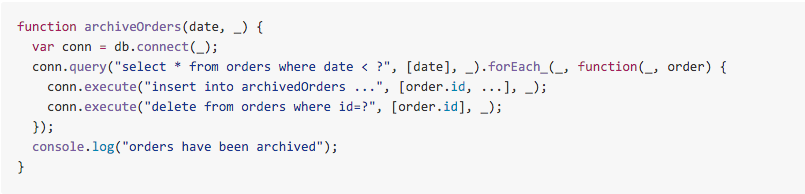
\includegraphics[scale=0.5] {streamline}
\caption{Streamline uses an underscore to replace callbacks with synchronous-looking code}
\label{fig:callback-hell}
\source{https://github.com/Sage/streamlinejs}
\end{center}
\end{figure}

Promises are a concurrency primitive that essentially ``promise'' that a value will be there when you need it or fail entirely. The returned value of an asynchronous function is a promise, which is ``thenable'', meaning that a method can be called on it with the resolved promise value as the argument. In English, one might describe promises as ``return this value, then operate on it.'' To make this design clearer, Figure \ref{fig:promises} is a code excerpt of how code with callbacks might be transformed with promises.

\begin{figure}[h]
\begin{center}
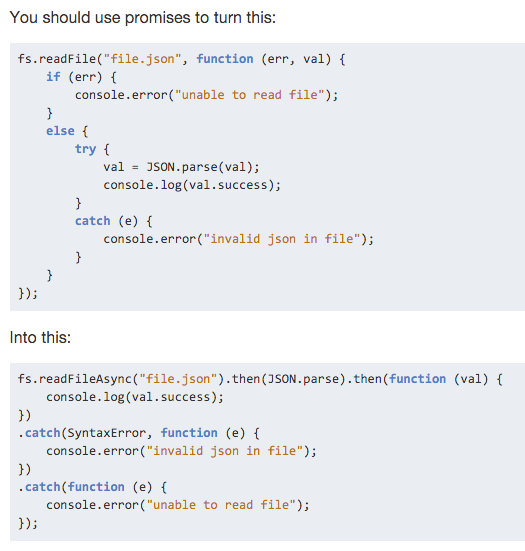
\includegraphics[scale=0.5] {promises}
\caption{Promises help with writing flat code}
 \label{fig:promises}
\source{bluebirdjs.com}
\end{center}
\end{figure}

After evaluating the two approaches on such metrics as popularity, readability, and functionality, we decided to use Promises, primarily because they will become part of the Javascript language in its next official release, ECMAScript 6. With promises as a core language feature, we judged it to be more likely that a Javascript developer would understand our code without needing to consult dense reference documentation.

Once we settled on Promises, we had to choose a promise library, either a third party library or the standard Javascript library, which contains a beta version of promises. Among the most commonly used libraries are Q, D, and Bluebird. D lacks useful features beyond the core promise implementation so we ruled it out first. Both Bluebird and Q have extensive reference documentation. We found that due to Q's error handling, exceptions can go unobserved at the end of promise chains. Bluebird reports all errors without special syntax and displays helpful stack traces for error detection. In addition, Bluebird has zero overhead abstraction, meaning that we can use its features without sacrificing performance. Bluebird emerged as the best option, also providing helpful methods for operating on promise values (for example, with a map() function) in line with promises chains. In our implementation, we make frequent use of Bluebird promise chains in which each step in the chain returns a promise. Every asynchronous API wrapper method we wrote returns a promise. Any time we call an asynchronous method, including database queries and wrapper method invocations, we wrap the return value in a promise handler to keep our code flat.

\subsection{Documentation}

In order to enable general-purpose use of our API (and to facilitate our front end development process), we needed to document it. Our goal was to inform API clients of the exact parameter requirements of each API method and the expected return values, establishing the contract between caller and callee. Along with the option of writing a Github wiki, Swagger and apidoc emerged as industry favorite Node packages to generate documentation. With Github, the documentation is included with the project code, a benefit for convenience. However, Github's editing platform for project wikis makes it difficult to include JSON samples, which are essential for describing HTTP request body syntax. Swagger produces a clean, readable documentation page as its end result, but creating that page requires using Swagger's own editing tools. At this point in the development process, we had already written many of the API endpoint methods, so it would have been burdensome to retroactively conform to Swagger's format. Apidoc, on the other hand, allows you to create API documentation with Javadoc comments directly in the file. You can include JSON samples easily, and generating the documentation page is one command line instruction to compile the Javadoc comments. The created page is interactive, legible, and visually appealing. Considering these tradeoffs, we decided to use apidoc, and host the generated documentation page using Github pages, a free web hosting service to associate a website with a Github project. For each API method, we wrote a Javadoc comment to specify endpoint descriptions, required parameters, return status codes, and example JSON request and response bodies. The documentation can be found in its entirety at \url{http://g2-iw.github.io/backend-iw/}. With the API fully documented, the back end services can operate independently of the Android app. The SolarSource app is just one client of the API; anyone can use the back end services to determine the viability of a rooftop solar installation.

\subsection{Database Layer}
For the purpose of returning a recommendation, it is not strictly necessary to store home objects. The back end could simply perform the evaluation from start regardless of whether the home has been profiled before. However, we wanted to leave open the possibility of using performance data from profiled homes (i.e. a homeowner installed panels after evaluating the SolarSource recommendation) as part of the crowdsourced platform to inform future recommendations. In addition, we recognized that the third party API requests are costly - if we had already performed an analysis for a home it would be unnecessarily time consuming to go through the process again for the same home. We therefore chose to store home objects in an application-attached database. Implementing that decision required choosing a database. Our goal was to make database operations as seamless as possible given that they were used as a performance improvement and not a core component of the analysis. We were also guided by time-to-learn (based on documentation, peer reviews, and past experience) and code simplicity. Possible approaches included MongoDB, Hadoop, and Redis. We chose MongoDB because it uses JSON-like documents to store database entries rather than relational tables. The JSON documents are compatible with regular Javascript code without much processing. With MongoDB we were also able to use the Node.js library, Mongoose, which supports promises. We created a MongoDB database and connected it to the application, wrote schema files to describe the structure of home database documents, and wrote database query and document creation code in the route handlers.

\subsection{Deployment}
Our goal in this stage was to deploy the API to a stable, reliable server that supports external volume storage. We opted to deploy to a cloud server because of simplicity and low cost. Several approaches exist for deploying an application to a cloud server, including Amazon Web Services (AWS), Digital Ocean, Heroku, and Google App Engine. We chose AWS because it allows free deployment under a certain usage limit and provides an instance machine image preloaded with the Node.js and MongoDB environment. We set up a security group to allow all members of the SolarSource team to SSH into the cloud instance. We then generated a key pair for encrypted sign-in. We launched an Elastic Compute Cloud (EC2) instance with the desired machine image. After developing and testing the API locally, we pulled the code from Github on the cloud instance, configured the production database, and started the server with the Node.js forever library, which keeps the server running after you break the pipe with the remote instance.

\subsection{High Level Process Flow Overview}

\begin{figure}[h]
\begin{center}
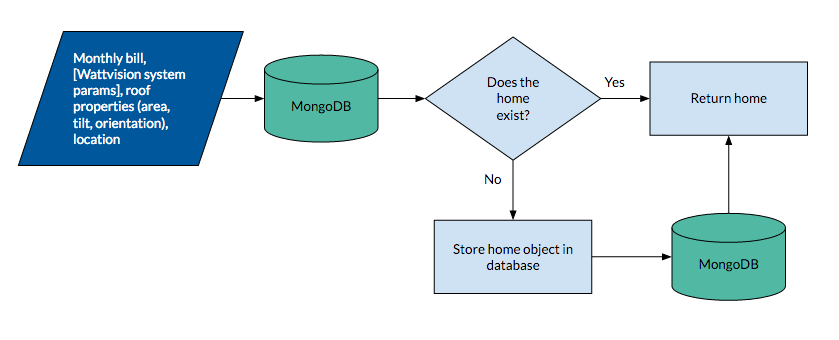
\includegraphics[width= \textwidth]{POST}
\caption{Home creation POST method}
\label{fig:post}
\end{center}
\end{figure}

\begin{figure}[h]
\begin{center}
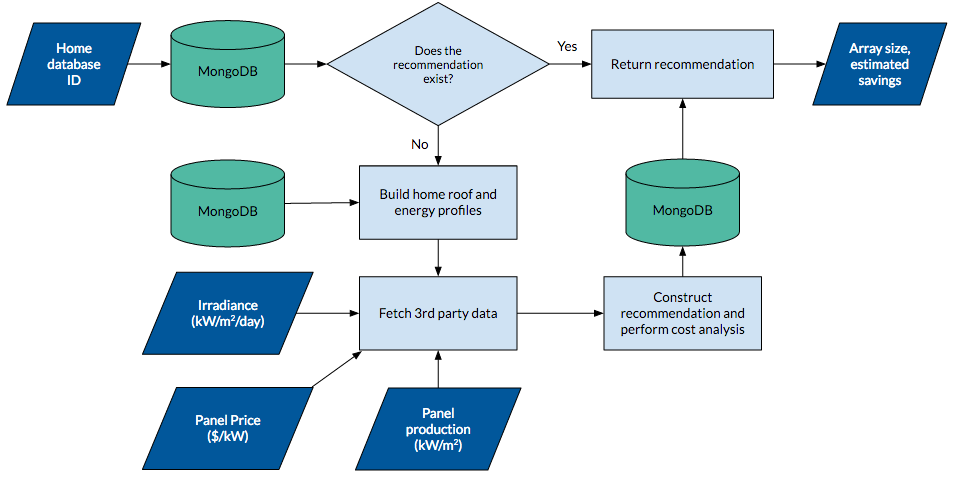
\includegraphics[width=\textwidth] {GET}
\caption{GET route to retrieve recommendation and cost savings estimate}
\label{fig:get}
\end{center}
\end{figure}

We first outline the flow of control to generate a recommendation and cost savings estimate for a home. Please see Figures \ref{fig:post} and \ref{fig:get} for graphical process illustrations. The process begins with an HTTP POST request. The input to our system is home energy consumption (in dollars per month), optionally the Wattvision system identification number, and the roof properties: usable area, tilt, orientation (compass direction), and azimuth angle. All inputs are passed in the body of the request. In the handler method for the POST request route, we store the home in the database if it does not yet exist and return the created home JSON object. 

To access the recommendation for that home, the client then makes a GET request to the recommendation endpoint, passing the home's database ID as a query parameter. If the home's recommendation has already been computed, the route handler returns the existing recommendation. Otherwise the method constructs the home profile from the user data and retrieves the necessary information from third party APIs. It then passes all the necessary information to the recommendation engine module. The recommendation engine computes the recommended solar array size and performs the cost comparison analysis. The router formats the recommendation and returns a JSON object to the client with the recommended array size and estimated savings. Figure \ref{} shows a sample JSON output. The following subsections describe each of these steps in detail. We separate the home creation endpoint from the recommendation retrieval so that a user can easily access the recommendation of a previously used home without the unnecessary steps of the POST creation method.

\subsection{Home Creation}
In the first stage, the client makes a POST request to the API. Our goal is to convert the user-passed JSON object into a home database entry and store it in the database. The input, as mentioned before, is the monthly electricity bill and roof properties. For this simple handler, our approach is largely determined by our decisions to use MongoDB and promises. However, there is freedom in our choices of file layout and parameter passing. One approach is to mount the handler function directly onto the main route of the application. This would be done in the {\em app.js} file, which starts the server and configures the application properties. Another common Express approach is to create a separate router file (a module), and append route handler functions to the router module. In the {\em app.js} file, you mount the entire route onto the application rather than the individual methods. 

We chose the latter approach for two key reasons. Firstly, it is less error prone; rather than writing the same style code to mount multiple methods in the same API endpoint group, we only need to mount the router once. Using the router modules has the added benefit of clarifying the API structure; each router has a one-to-one mapping with an endpoint group. The router modules effectively package up related route handlers. Secondly, it encourages decoupling of components. In this and other aspects of the codebase we strive to decouple components to the largest extent possible. Decoupling enables easier module swap-in and modification without breaking other parts of the code; service components can be swapped out without changing the routers at all, so long as they use the same parameters. A potential workaround to this parameter problem is performing no input validation in the router and sending a full Javascript object to the service or database layer as an argument (in that case, the home database schema would be a generic and mutable empty object. Service layer code would have the responsibility of retrieving the necessary fields from the home object. We opted not to do this because it risks safety - the user can pass anything in a request body. We preferred a strict structure for the home database schema to enable MongoDB to perform internal input validation.

We created a separate router for the CRUD  (creation, retrieval, update, and deletion) route handlers. Although most of these methods are not accessed by the Android application, they facilitate testing and could prove useful for general API access. Figure \ref{fig:postrouter} shows the route handler for the POST method.

\begin{figure}[h]
\begin{center}
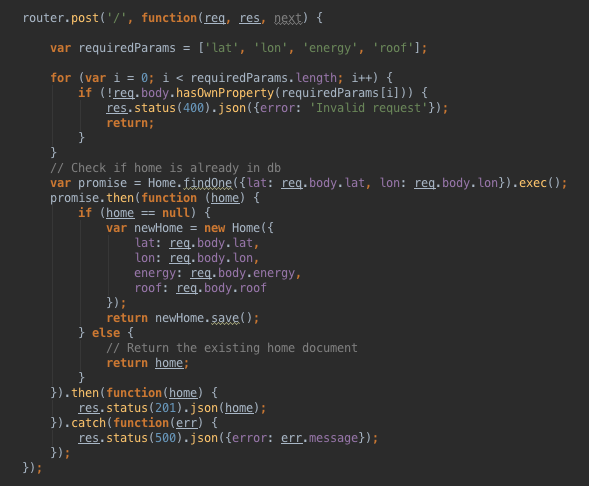
\includegraphics[scale=0.6] {postrouter}
\caption{Route handler for home POST method}
\label{fig:postrouter}
\end{center}
\end{figure}

We first verify that the caller has supplied the required parameters. Using promise syntax, we first query for the home in the database by latitude and longitude in case it has already been created. If so we retrieve the database entry and return it immediately. Otherwise we create a new home document with properties equal to the request body attributes. We then save the home in the database and return the database entry to the caller to indicate to indicate the process was successful.

In this and all other HTTP methods, we strictly adhere to the model of: perform input validation, query the database for an object or create a new object, and return a JSON object to the user, either an error description or the result of the successful database operation.

\subsection{Recommendation and Cost Analysis}
In the second stage, the client makes a GET request to the recommendation endpoint, using the database ID returned in the POST response body as a query parameter. If a recommendation has not been created for this home before, then it begins the analysis. The overall goal of this stage is to return an accurate recommendation for an array size to cover a percentage of consumption and estimated cost savings by installing the recommended array. The inputs to this stage are home energy and roof profiles, solar irradiance, panel price, and array generating capacity, the latter three of which come from third party API requests. We will discuss each step individually. For the overall structure of the recommendation route handler, a common approach for a handler that makes many asynchronous requests is to use nested callbacks. However, that option contradicts the design goals from our approach. This is an ideal use case for a Bluebird promise chain. At each step in the process, we retrieve data that ultimately gets passed to the constructor of the recommendation engine module. The promise chain ensures that the data is available when the engine object is instantiated. The promise chain also allows us to write flat, readable code, with each component of the promise chain performing a well-defined task. Rather than using global variables to store the result of each external method call, we used one context variable, a Javascript object, bound to the promise chain. At each stage we append a new attribute to this dictionary object.

The recommendation route handler illustrates how we separate HTTP routing from the analysis tools entirely, adhering to our decoupling principle. The logic is abstracted away in the service and model levels, while the router performs the necessary linkage operations.

Implementation: bluebird promise chain + break up components
alternative 

\subsubsection{Construct Home Models}
Goal of step: analyze user-passed values to produce necessary values for recommendation
Previous approach: inline the analysis

The goal of this step is to construct models for home energy consumption and roof availability using data passed by the client in the first phase. The models provide access to properties required for third party API calls and cost analysis. Such properties include total usable available roof area and average monthly electricity consumption. In the simple case, the data from the user is sufficient for the profiles. One possible approach, therefore, is to simply retrieve the necessary attributes from the home database entry. An alternative is to create separate modules for the roof and energy profiles and only provide access to the necessary data through an interface. 

We decided to use the latter approach in anticipation of adding methods to operate on the user-inputted data for more advanced analyses. For instance, if the user grants access to his Wattvision data stream, we could construct an energy model to analyze patterns of consumption. Rather than using data straight from the home database object in our recommendation algorithm, we retrieve home information only through the models' interfaces. That way, we can do more advanced computation behind the scenes without changing the calling code and still return the necessary information to the caller through {\em getEnergyProfile()} and {\em getRoofProfile()} functions.

In the recommendation route handler, we call the constructors for the energy and roof models, passing in the matching objects from the home database objects and, in the case of the energy mode, the Wattvision data stream. We choose to fetch the Wattvision data in the recommendation handler (rather than, say, the energy model itself) because we wanted to have all external API requests in the same place. This helps prevent potential asynchronicity issues. The model constructors call the analysis methods so that the caller can simply call the constructor.

The roof model comprises such properties as square footage, roof tilt, shade coverage, and geographical coordinates (to ascertain azimuth angle). Information from the roof model determines the physical constraints for an installation and subsequently the maximum power generation. For the energy model, we perform an analysis using measurements taken by the Wattvision sensor if the home has one. Otherwise we simply store the monthly consumption value by dividing the monthly cost by the standard dollar per kilowatt-hour cost retrieved from NREL's Utility Rates service. The home's electricity use determines the required array size to cover a portion of the home's consumption. In our current implementation we recommend an array to cover close to 100\% of the home's consumption. However, we provide the flexibility to change that percentage in a configuration file or plug in a custom tool to determine the most cost effective installation size given patterns of usage or electricity price forecasts. At this step we have the maximum size of the array and the required array production to match a specified consumption amount. 
After the constructor calls return the recommendation route handler retrieves the home and energy profiles through the model interface methods and append the profile objects to the context variable.

\subsubsection{Retrieve NREL Data}
Goal of step: get the NREL data to perform the analysis
Alternative approach: inline the API calls

In the next step, our goal is to retrieve the necessary NREL data to generate a recommendation and perform the analysis. We wanted to do this in a way that did not disrupt code readability. The required inputs are the home's coordinates. The desired outputs are price of panels, average solar irradiance at the coordinates (kWh/m2/day), and panel production (kW/m2). We discuss acquiring panel production in the next section.

In this step we face the issue of calling external NREL API endpoints. One approach is to call each method directly when needed in the route handler. However, that would require complicated callback logic and entangle the router logic with boilerplate HTTP requests. We took an alternative approach; we created entirely separate modules for calling external API methods. In these modules, we have a separate method for each endpoint we need to hit. We use the Node.js library, superagent, to make the requests. Superagent provides simple syntax for specifying query parameters, request headers, and response format. These methods each return a Javascript promise object to facilitate integration into the promises chain. With this approach, our route handler calls a method from the wrapper module in one-line and receives the formatted response with the necessary data. Figure \ref{fig:nrel-wrapper} shows an example of one wrapper method for the NREL Solar Resource API and how it gets called in the route handler:

\begin{figure}[h]
\begin{center}
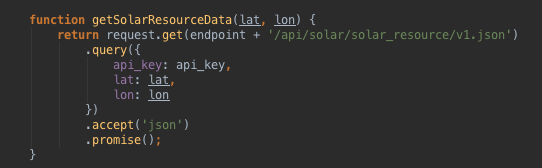
\includegraphics[scale=0.6] {nrel-wrapper}
\caption{Wrapper function to make HTTP request to NREL API}
\label{fig:nrel-wrapper}
\end{center}
\end{figure}

\begin{figure}[h]
\begin{center}
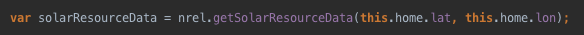
\includegraphics[scale=0.6] {nrel-call}
\caption{Wrapper function call in the recommendation router}
\end{center}
\end{figure}


\subsubsection {Acquiring Generation Data}
Perhaps our most difficult challenge was how to accrue accurate solar panel generation data. Our approach calls for the use of actual data in place of fixed values to compute the power per area of a hypothetical array. The two types of generation data are static and dynamic. Static data is normally downloadable, a spreadsheet of generation values over a certain time period. Dynamic data is retrievable in real time via API request. It provides the current power production of the solar array. We opted to use dynamic data to avoid bloating the codebase with large data files that would need to be manually updated periodically. With dynamic data, we can make on-demand HTTP requests and use the data when it is needed during the analysis. The application does not store the data, instead incorporating it *on the fly*. Our options for dynamic generation data were severely constricted by what we could get permission to use. Often generation data is proprietary and protected. Given our extensive use of NREL's services, we reached out to them to try to gain access to data sets. After speaking with Principal Scientist Sarah Kurtz, we were given an API key for the Photovoltaic Data Acquisition (PVDAQ) service, which provides access to PV performance data collected by NREL for systems throughout the country. Endpoints of the service return generation data for each site including monthly generation, peak power output, site elevation, site location, array area, and DC power readings at regular time intervals similar to Wattvision meter readings.

In our implementation we query the PVDAQ database for systems closest to the target home. We take an average of power per area across a collection of PVDAQ systems for the value that gets used in the analysis.

Most of the PVDAQ systems are large commercial installations. Even though the total size of the installation should not effect the power per area value, we thought it would bolster the reliability of our recommendation if we also used generation data from residential solar arrays as part of a sort of *crowdsourced* platform. From our survey of related work, we selected Enphase as our target system for generation data. The Enlighten API has well-documented endpoints to access site metadata, current production in 15-second intervals, and total monthly production. We reached out to Ben Smith on the Enphase developer team and requested access to Enlighten system data. After walking us through the process of creating an Enphase application, Mr. Smith identified candidate systems he thought would be representative of actual generation in Long Island, New York, where we would ultimately conduct our evaluation experiment. Mr. Smith is waiting for company approval to send out emails to the owners of those systems, in which we described the purpose of our project and requested access to their API keys so that we could make requests on their behalf. At present we are not using the Enlighten system data, but the code support exists to integrate those data feeds into the analysis once we gain authorization from the owners. Figure \ref{fig:enphase} is an image of the email that the candidate owners will receive from Enphase:

\begin{figure}[h]
\begin{center}
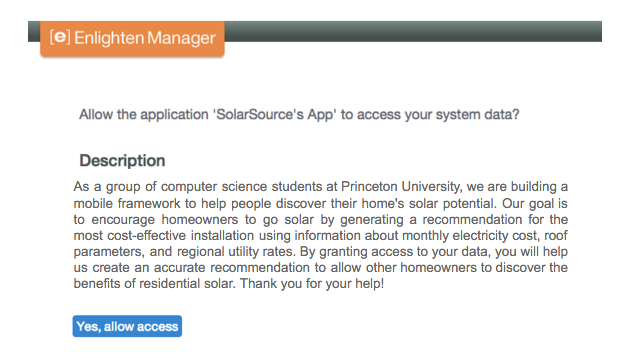
\includegraphics[scale=0.4] {enphase-access}
\caption{Authorization page sent to Enlighten customers}
\label{fig:enphase}
\end{center}
\end{figure}

\subsubsection{Calculate Recommended Array Size}
Goal of step: use data to calculate the array size
Approaches: one big method

We use values from the energy and roof models as query string parameters for third party API requests. To convert from required array production to array size, the first step is determining how much sunlight the home receives. We make a request to NREL's Solar Resource service, which returns an average irradiance value based on the location, orientation, and tilt angle of the roof (parameters retrieved from the roof model) in units of kWh/m2/month. Next we have to compute the array's presumed production in kW/m2. For that we rely on the actual generation data from the PVDAQ and Enphase sources close to the target address. At this point we know the array size and maximum capacity to generate the required amount of electricity. Here is the formula we used:

\[ \mbox{array capacity} = \mbox{total consumption (kWh/month)} * \mbox{desired percentage coverage} / \mbox{average irradiance (kWh/$m^{2}$/month)} * \mbox{average power (kW/$m^2$)} \]

\subsubsection{Perform Cost Comparison}
Goal of step: perform cost comparison
Alternative approach: 

To determine the cost savings, we first compute the 20-year electricity costs assuming the home uses only grid electricity. For this we use the monthly cost the user provides or the product of monthly consumption from a Wattvision analysis and cost per kWh retrieved from the NREL utility rates endpoint. We can either use a fixed value for assumed electricity price and consumption increase (set in a configuration file) or call a method from an external module. To calculate the cost of the array, we call NREL's OpenPV endpoint to get the current price of a panel (in units of \$/kW) and multiply it by the array capacity. Then we break up the total cost into 20-year loan payment periods. For the loan APR rate, we can use a custom projection tool or a fixed value. In this iteration we assume that electricity generated but not used can be sold to the grid at the same price it is purchased for, as is the case in California today. That way it doesn't matter if the home doesn't have an energy storage system; the grid serves as a battery and the electricity purchased from and sold to the grid cancel, so the only cost is the monthly loan payment. If the hypothetical array does not cover all of the home's consumption, we also include the balance for grid electricity cost. We produce the cost-savings estimate by taking the difference of the aggregate grid electricity costs and the price of the solar array (purchased with a loan). Here we accept that modern solar arrays use micro-inverters and should require no maintenance (and therefore no additional cost) during their first 20 years. We return to the client a JSON object in the following format:

\subsection{Modular Architecture}
A central challenge throughout the development process lay in taking advantage of the modular architecture. More specifically, we wanted to enable easy swapping-in and swapping-out of components. One option was to encompass large portions of the logic within long functions. However, we realized that each component of the analysis could potentially call for its own tool. As a result, we decided to break up the logic into small, well-defined parts. For example, in our calculation of estimated cost savings, we use 4 methods, each with a well defined task:

The principle of decoupling extends to within the files as well. 

\begin{itemize}
\item calculateArraySize()
\item calculateArrayCapacity()
\item calculateArrayCost()
\item performCostComparison()
\end{itemize}

\subsection{Testing}
We tested the API endpoints using the Postman HTTP client, which allowed us to specify headers, query parameters, and POST request body in a nice format. Postman displays the response JSON object and any status codes, as shown below.

FIGURE

\subsection{Evaluation}
\begin{itemize}
\item Experiment design...
\item Data...
\item Metrics...
\item Comparisons...
\item Qualitative results...
\item Quantitative results...
\item Further results needed...
\end{itemize}
We used two methods to test our approach. For both methods we used NREL's PVWatts service. PVWatts estimates the performance of hypothetical residential and small commercial PV installations given installation properties like tilt, latitude and longitude, tilt angle, and nameplate system capacity. The returned JSON object contains three arrays: monthly irradiance values (strength of solar energy at the location), monthly DC array output, and monthly AC array output. When making calls to the service, we had to make certain assumptions due to lack of available data. PVWatts requires the caller to provide the module type (standard, premium, or thin film), and system losses. We assumed a standard module and 5\% losses.

Our initial goal was to provide the homeowner with an accurate framework to evaluate a rooftop solar array's potential to generate electricity and save money on the electricity bill. In our evaluation we sought to test the accuracy of the framework's recommended generation and cost savings. To evaluate how well we achieved our goal of generality, we perform a qualitative analysis on several key principles.

For our first evaluation method we surveyed a home in Princeton with solar panels already installed. 

**
Comparing the actual electricity bill (obtained from PSEG) to the projected costs if the homeowner had used our recommendation, we determined if the framework would actually save the user money. 
**

Using past electricity bills we extrapolated to compute cost savings due to the solar installation. For that we took the difference between average monthly consumption before panels and consumption after the panels were installed. We had an admittedly small sample size considering the panels were installed last March. We manually mapped out the roof area, then used that data to produce an installation recommendation with our framework. By passing the installation specifications as parameters to NREL's PVWatts performance prediction service, we estimated the cost savings of the hypothetical array if purchased with a 20-year loan. Finally we compared the predicted savings to the extrapolated actual savings. We chose cost as the primary evaluation metric because our goal is to convince homeowners that solar energy is a cost-effective alternative to utility electricity alone. Concern for the planet's wellbeing will not drive widespread change in electricity generation. We must appeal to the homeowner's economic interest if we want to expand solar. One home is of course a small sample size for our evaluation. We were limited by access to electricity billing data for homes with panels already installed. In future work, we would use this evaluation model on a wider scale. After performing the analysis, here are the results:

The extrapolating actual cost savings reports total 20-year savings of \$19000. The SolarSource recommendation yields expected savings of \$15000, an error of 21\%. Although it is high error, we must keep in mind that the service provides a ballpark estimate. Its main goal is to get people aware of their rooftop generating potential. We think savings on the order of \$15000 are likely to do that. We hope to use the results of this small evaluation to inform future iterations of the recommendation analysis.

The second evaluation method was to test directly against Project Sunroof. We chose Project Sunroof because it is a direct comparison application that motivated the development of SolarSource. To isolate evaluation of the back end API, we used Project Sunroof's own rooftop mapping for each home. We ran the SolarSource algorithm and Project Sunroof algorithm on 20 homes in Long Island, New York. For each home we used the actual monthly electricity bill. Even though we identified monthly consumption as an unspecific metric, it is the only option for Project Sunroof. We therefore judged it appropriate to use in the direct comparison. The two services yield recommended array sizes and 20-year savings. We used 20-year savings because it is the only option provided by Sunroof. Here are the results from the analyses, where each point represents one home. The X-axis is electricity bill and the Y-axis is estimated 20-year loan savings. We also include the recommended array size in kW. For privacy concerns, we omit the addresses. 

Again we made use of the PVWatts API, passing the installation specifications as parameters. We compared the predicted performance of each array to the estimated performance reported by the two frameworks. PVWatts returns an array of monthly AC electricity outputs for the array. We take the average of these values as the array's monthly production. To ascertain generation of the recommended array, we multiply the home's monthly electricity consumption value by the percentage of consumption that the array purports to cover. We can also compute the PVWatts predicted savings by multiplying the average monthly consumption value by the price of electricity, adjusting for expected price increase, using the assumption that the homeowner saves whatever they don't purchase. We then calculate the error of framework-expected 20-year savings and PVWatts predicted-savings for each surveyed home.

 In Figure 4, we show the monthly output values for SolarSource, Project Sunroof for each surveyed home and provide the percent error compared to the PVWatts simulation. Figure 5 shows the cost comparison.
 
 (two graphs, 1 shows production estimates for PVWatts, Sunroof, and SolarSource, other shows cost savings for each home)
 
 (one table, small summary of cost comparison taking the average from the previous graphs)

A limitation of this approach is that SolarSource relies heavily on NREL services, which PVWatts may inherently be closely aligned with. A more objective comparison might use SolarCast to predict future performance. However, as SolarCast is still under development, we settled on PVWatts for the analysis. 


Among the twenty homes we tested, five of them had monthly electricity bills that exceeded Project Sunroof's maximum allowable value of \$500. Two of the homes were not covered by Project Sunroof at all and have been omitted from the direct comparison analysis.

From the data, Project Sunroof has a \% average error compared to the project performance from PVWatts. The SolarSource framework yields \% average error.

We also performed a qualitative analysis of SolarSource compared to Project Sunroof, using some of the key principles that guided our approach. Whereas Project Sunroof is only available in 10 US cities, our framework can be used anywhere with internet access as a result of the user-created roof and energy profiles. Whereas Project Sunroof does list its assumptions in the estimated savings calculation due to the array, our framework is open source. An interested user can examine the code on Github to learn how we perform the analyses. We strove to write self-documenting code with a clean structure and descriptive variable names to facilitate understanding.

Although we provide many of the same values at Project Sunroof, we differ in *how* we provide that information. Sunroof displays the information in the app's interface. Though visually appealing, the format is inflexible. There is no Project Sunroof API to retrieve the data from the analysis. With a RESTful API backend, we return the information in a JSON object. 

A user can make an API request outside the Android application using an HTTP client like Postman or the curl program on the command line. All that is required is a valid JSON request object as specified on the documentation page. The roof parameters could come from a manual mapping (perhaps with a tape measure, as we used for the Princeton home).

The SolarSource Android application or any other client can make requests to the API using an HTTP client like Postman or the curl program on the command line. All that is required is a valid JSON request object as specified on the documentation page. The roof parameters may come from a manual mapping (perhaps using a tape measure, as we did for the Princeton home we tested on). The client can display or process the returned information however they please. We provide the analysis tools; we don't restrict how the client uses our output.

Project Sunroof cannot be modified or augmented by the open-source community. It uses fixed values for electricity price increase, APR, and future consumption. There is undoubtedly development underway at Google, but there's no way for developers to build on their framework. Google could fathomably open-source the code (the company has a Github organization with over 400 project repository) or release an API as part of its developer program. Currently, however, the code for Sunroof is hidden behind the interface. On the other hand, our code is intended to be *forked* on Github. The Node.js framework and our modular architecture enables developers to easily plug in their own modules. Rather than using a fixed value for the assumed electricity price increase, a developer could build her own price forecast model and swap it in to the analysis. Or instead of using the monthly electricity bill as the basis of the analysis, a developer could analyze the Wattvision data stream to determine heaviest hours of use. Without expertise on economic trends or data analytics, we couldn't build advanced models ourselves. But we could create opportunities for people well-versed in those topics to create tools of their own. Our modular architecture and open-source codebase permit that. Figure \ref{fig:qual} is a chart summarizing the qualitative comparison between SolarSource and Project Sunroof.

\begin{figure}[h]
\begin{center}
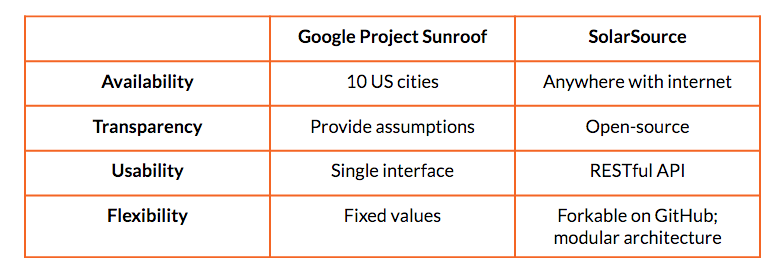
\includegraphics {qual-analysis}
\caption{A qualitative comparison between SolarSource and Project Sunroof in 4 key categories}
\label{fig:qual}
\end{center}
\end{figure}


\subsection{Summary}
\begin{itemize}
\item Conclusions...
\item Limitations...
\item Future work...
\end{itemize}

We presented SolarSource, an open source framework that recommends to homeowners a cost-effective solar installation. We also discussed several use cases where our RESTful API can be effectively used. No individual step in our analysis is novel. The combination of solar performance and public weather data and the application of modular architecture to a solar potential API are the main contributions of our work.

Our hope is that our framework can help homeowners unlock the potential of rooftop solar. Our implementation takes advantage of mobile technology, which allows to user to build the profile of the home so that the framework can be used anywhere. We leverage 3rd party APIs to provide a recommendation for a solar array, informed with crowd-sourced generation data from actual arrays. Finally we report the result of our analysis, composed of the recommended array properties and estimated cost savings, to the user.

The accuracy of our recommendation is limited by our access to atmospheric weather data. For Project Sunroof, Google is able to leverage its proprietary data in historical cloud and temperature patterns that might affect solar energy production. We were limited to public data from sources like NREL. In future development, we would look into bolstering the accuracy of our weather information.

One limitation of our approach is that it only works for a single, continuous installation. It cannot account for multi-part roofs that face different directions or have different tilt angles. In future work, we would adapt the framework to allow disconnected roofs with different properties.

Another limitation is that we assume that the panels would be purchased via loan, such as Solar City's MyPower program. In actuality, the homeowner could also lease the panels or buy them outright. Building support for various financing options is another key component of our future work.

Enphase Enlighten and PVDAQ both require developer accounts with unique API keys, which we store privately. A developer who forks the SolarSource project on Github does not have API access to either service. In order to enable further development on the project by outside contributors, we must find a workaround to this issue. One potential solution is to store the PVDAQ data statically in a file that we update periodically (once per month, for instance). We don't envision the Enphase data will ever be accessible publicly given that we needed special access from the user to make API requests on his or her behalf. Unlike PVDAQ, we couldn't store the data within the app; In the access authorization email we specifically stated that the user's system generation data would never be published.

Because we chose not to use map APIs for the roof profile, we rely on the user to provide the tilt angle of the roof and azimuth angle relative to the sun's path. This approach places a large burden on the user to compute the correct values. In the next iteration, we would look for techniques to calculate those values on the back end.

In our evaluation, PVWatts only accepts latitude and longitude values with precision to the nearest degree. This is a limitation because many of the homes we tested were all in the same area, a necessary decision in light of limited access electricity billing data and Project Sunroof's coverage.

Once the SolarCast API is completed we intend to use it both for evaluation and as part of the recommendation algorithm. Rather than assuming the panels will generate electricity at the same capacity for their lifetime, we could incorporate SolarCast's future prediction algorithms to get a more finely-tuned view of lifetime generation potential. That measure would improve the precision of the cost-savings estimate.

Incorporating SolarCast is just one step in improving the algorithm. In future work we would continue to refine our prediction schema, seeking the most accurate methods to compute power production as well as average irradiance. We will be presenting the framework and our results to NREL in late January. The director of the PV program is interested in how developers use the NREL API. She sees SolarSource as an ideal example use case and invited us to demo the app for her colleagues at the NREL headquarters in Golden, Colorado.

Wattvision expressed interest in integrating SolarSource with its existing software suite. Although we intend for the framework to remain general and open source, we could build out a customized version for Wattvision. With that in place, the SolarSource recommendation would be displayed for any Wattvision customer who opts in to discover the cost savings potential of a solar installation.

\subsection{Acknowledgments}
We are extremely grateful to Alan Kaplan for his guidance and constant support throughout the project. We'd also like to thank the Princeton University School of Engineering and Applied Science for its generous funding and the Blejwas family for allowing us to survey their home for testing purposes. We are particularly appreciative of the efforts of Sarah Kurtz at NREL for granting us access to the PVDAQ service and Ben Smith at Enphase for compiling a list of candidate systems and requesting API access on our behalf from Enlighten customers.

\bstctlcite{bstctl:etal, bstctl:nodash, bstctl:simpurl}
\bibliographystyle{IEEEtranS}
\bibliography{references}

\end{document}

